En primera instancia, se debe decidir cómo se quiere plantear la infraestructura de red, si vamos a construir nuestras propias torres, si por el contrario,vamos a funcionar como una operadora virtual, o si por el contrario, vamos a comprar a instalar nuestros propios equipos. En nuestro caso, nos hemos decantado por alquilar las torres de telecomunicaciones existentes, en las cuales vamos a instalar nuestros propios componentes. De esta manera, lograremos diseñar una red que cumple con compromisos económicos y, que a la vez, nos proporcionan cierto control en caso de averías o problemas.\\

Luego, debemos conocer dónde se encuentran las torres de telecomunicaciones existentes. Existen varias páginas web a través de las cuales podemos conocer dicha información, como Infoantenas \url{https://geoportal.minetur.gob.es/VCTEL/vcne.do}, un servicio desarrollado por parte del Ministerio de Asuntos Económicos y Transformación Digital, o AntenasGSM \url{https://antenasgsm.com}. A través de dichas páginas hemos podido conocer la localización de las torres, mostradas en la figura \ref{autovia}.\\

Sin embargo, tras seleccionar el modelo de estación base y antena que vamos a utilizar, en función de sus distintas características técnicas hemos propuesto un diseño de infraestructura, en la cual no va a ser necesario utilizar todas las torres de telecomunicaciones disponibles. Existen 11 torres desplegadas y utilizaremos 7 de ellas. En origen las distintas torres pertenecían a las propias empresas operadoras que prestan el propio servicio, o empresas filiales de las mismas. No obstante, la mayoría de ellas han vendido una gran cantidad de las torres a otras empresas, como pueden ser Cellnex Telecom, una empresa española, o American Tower Corporation, empresa estadounidense, ambas se dedican a la construcción y gestión de infraestructuras de telecomunicaciones. [Ref: Telefónica vende a ATC las torres de Telxius por 7.700 millones de euros | Empresas (elmundo.es) y Orange vende 1.500 torres a Cellnex para usarlas en régimen de alquiler | Empresas (elmundo.es)]. Se estima que el alquiler de estas torres se encuentra en torno a los 4.000 y 20.000 euros en zonas urbanas, y 1.000 y 15.000 euros en zonas rurales, costo que habrá que tener en cuenta a la hora de presupuestar la infraestructura.\\

Para el diseño del proyecto se ha contactado con los principales distribuidores en España de estos componentes, como pueden ser Ericsson, Nokia, Kathrein o Moyano Telsa, con el objetivo de lograr una red lo más similar a lo que nos podemos encontrar en las grandes operadoras españolas. Sin embargo, ninguna de estas empresas nos ha respondido ni nos has facilitado un catálogo de sus productos, por ello, hemos procedido a diseñar la red con equipos de los cuales si hemos podido encontrar información. \\

En primer lugar, hemos seleccionado una estación base proporcionada por una empresa china llamada Baicells, una compañía fundada en 2014 con sede en cinco continentes que ofrece productos de tecnología inalámbrica 4G y 5G. El modelo concreto es el Nova846, éste nos proporcionará una potencia de transmisión entre 0 y 37 dBm, una distancia máxima de 60km y una sensibilidad diferente en función del rango de distancias en el que se encuentra el usuario gracias a la modulación adaptativa.\\

\begin{table}[H]
\centering
\begin{tabular}{|c|c|c|}
\hline
\textbf{Esquema de modulación} & \textbf{RSRP {[}dBm{]}}            & \textbf{Distancia cubierta {[}km{]}} \\ \hline \hline
QPSK                           & -120 \textless RSRP \textless -110 & Entre 40 y 60                        \\ \hline
16 QAM                         & -110 \textless RSRP \textless -100 & Entre 10 y 40                        \\ \hline
64 QAM                         & -100 \textless RSRP \textless -85  & Entre 4 y 10                         \\ \hline
256 QAM                        & RSRP \textgreater -85              & Menor a 4                            \\ \hline
\end{tabular}
\caption{Cobertura en función de la modulación.}
\label{cobertura}
\end{table}

Dependiendo de la configuración proporcionará un rendimiento u otro, en nuestro caso nos hemos decidido por la configuración 6. Ésta nos brindará un rendimiento máximo en el enlace de subida, que nos interesa que sea máximo para que el mayor número de usuarios pueda enviar el vídeo en streaming. Lograremos tener las distintas capacidades mostradas para el enlace de downlink y uplink.\\

\begin{table}[H]
\centering
\begin{tabular}{|c||c|c|}
\hline
\textbf{Modulación} & \textit{\textbf{DownLink}} & \textit{\textbf{UpLink}} \\ \hline \hline
256 QAM             & 348 Mbps                   & 92 Mbps                  \\ \hline
64 QAM              & 264 Mbps                   & 70 Mbps                  \\ \hline
16 QAM              & 70 Mbps                    & 53 Mbps                  \\ \hline
QPSK                & 53 Mbps                    & 53 Mbps                  \\ \hline
\end{tabular}
\caption{Capacidades del enlace de bajada y de subida}
\label{capacidad}
\end{table}

La antena seleccionada es fabricada por la empresa irlandesa Alpha Wireless, una compañía fundada en 2006 dedicada a la fabricación de antenas. El modelo seleccionado es el AW3864-E-F, una antena sectorial de 4G que nos proporciona un ancho de haz de 65$\deg$ y una ganancia de 18 dB en las frecuencias de interés.\\

Con estos datos nos encontramos en disposición de simular la infraestructura, para ello hemos utilizado la herramienta de planificación y diseño de redes de telecomunicaciones Xirio-online. Una plataforma desarrollada una empresa española llamada Xirio, especializada en soluciones de ingeniería para telecomunicaciones. Con ésta se pueden crear mapas de cobertura y realizar simulaciones de propagación de señal con redes de telefonía móvil o televisión digital entre otras, así como evaluar del rendimiento de la red.\\

A través de un estudio de multicobertura e introduciendo todos los parámetros ya mencionados en la herramienta, hemos dispuesto las antenas a lo largo de tramo de autovía en las distintas ubicaciones en las que previamente localizamos las torres de telecomunicaciones. Como se puede apreciar en la figura \ref{xirio} teniendo en cuenta la cartografía del terreno, podremos cubrir la carretera a través de 7 estaciones base y 12 antenas. Asimismo, dado que no hemos logrado averiguar la altura exacta de cada una de las torres utilizadas, hemos supuesto una altura de 30 metros para todas ellas, ya que la altura media se encuentre en 15 y 50 metros.

\begin{figure}[H]
\centering
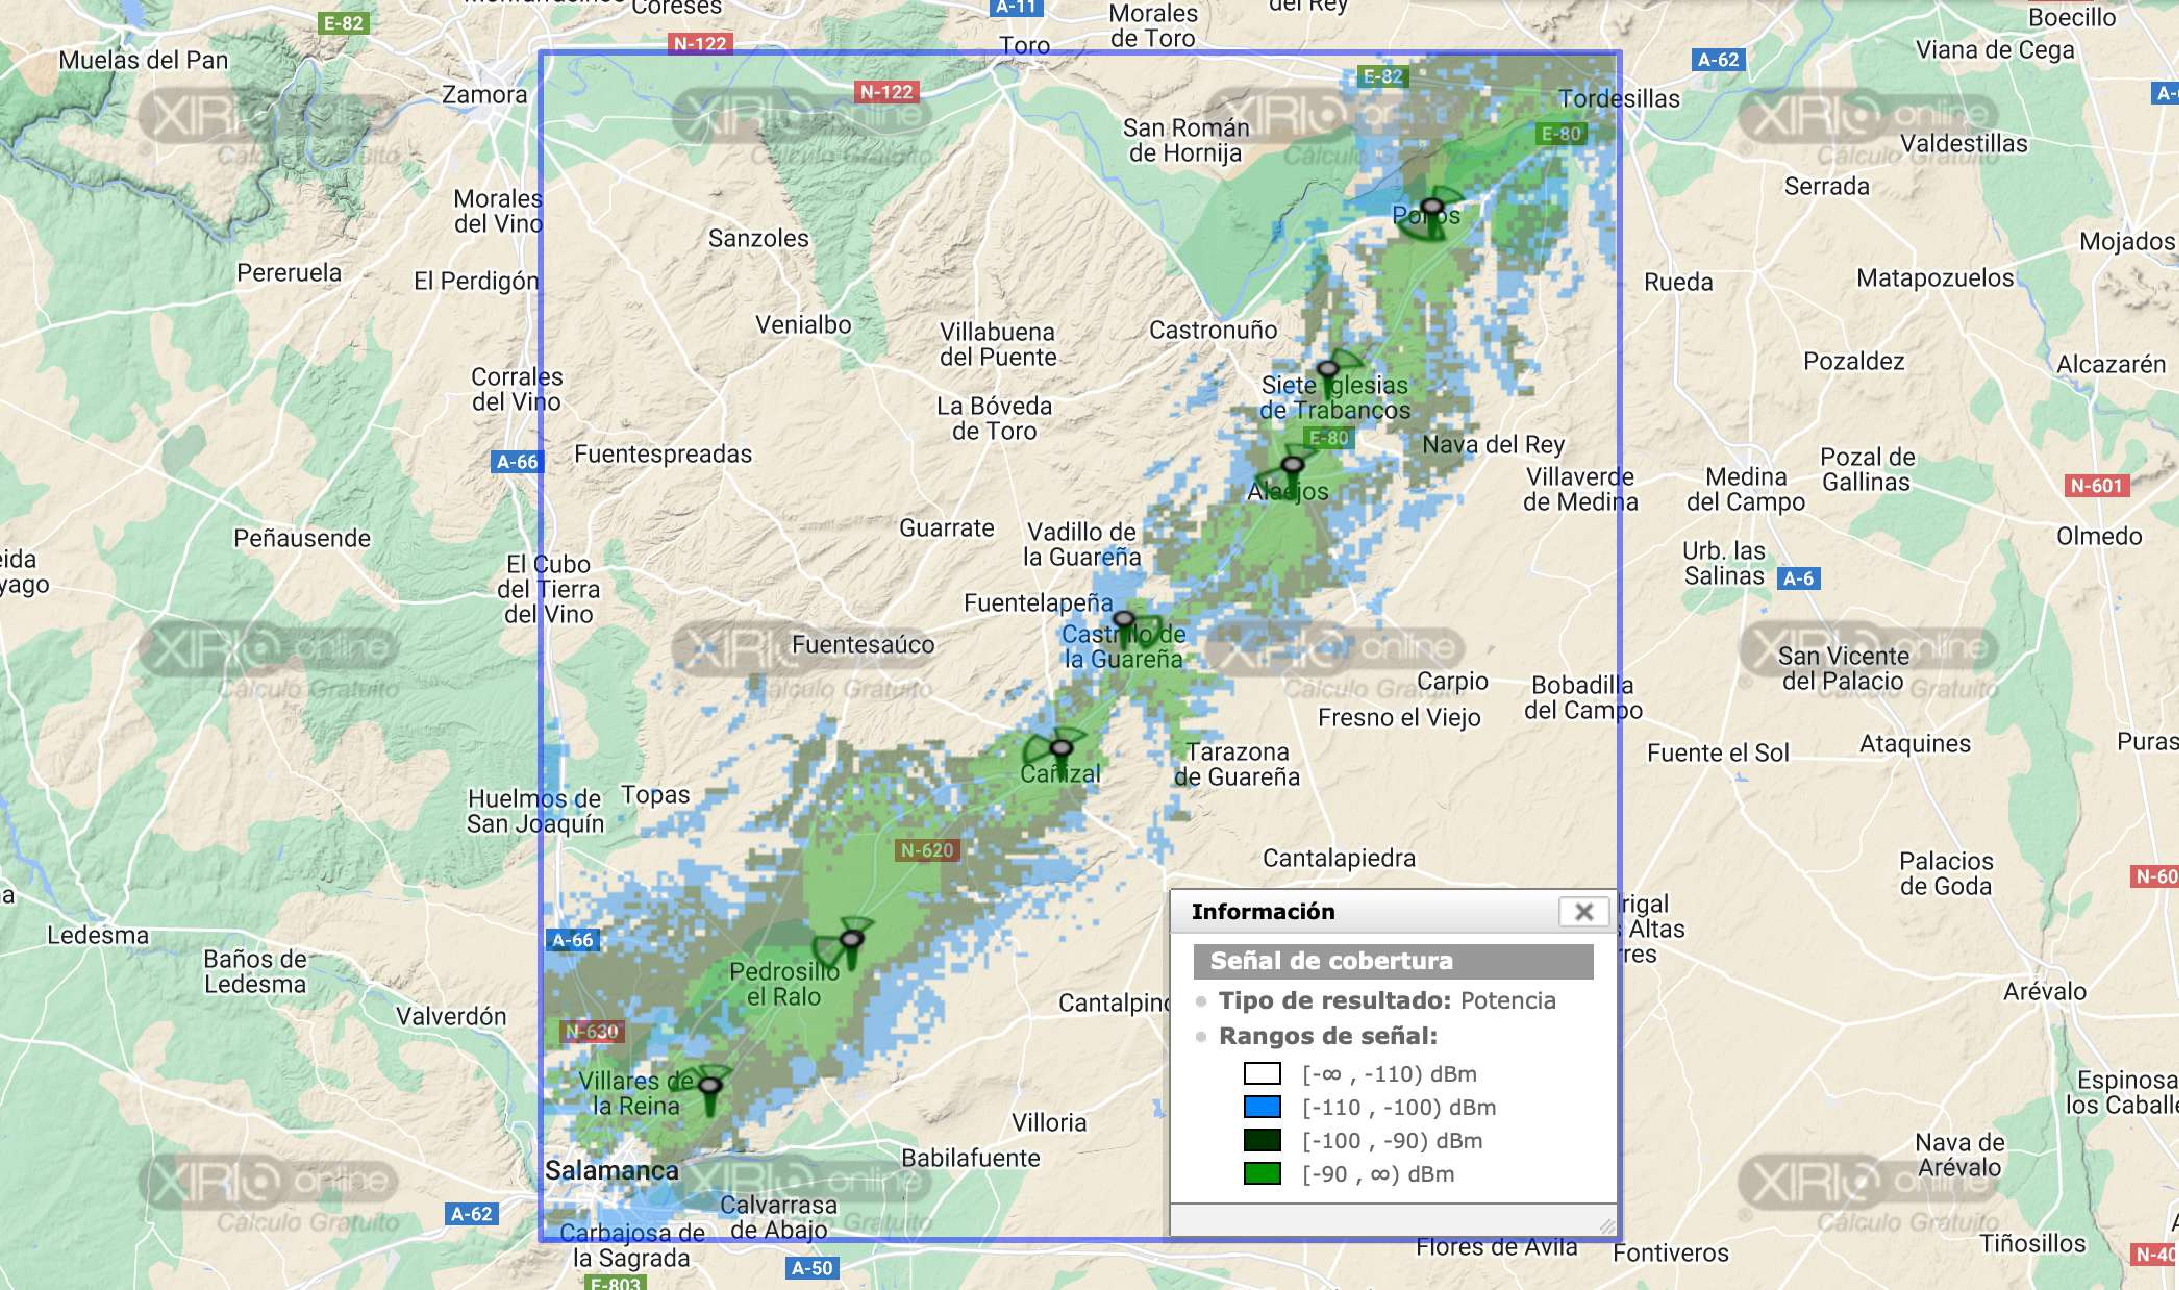
\includegraphics[width=\textwidth]{Imagenes/Solucion/xirio.pdf}
\caption{Distribución de la cobertura y estudio de cobertura}
\label{xirio}
\end{figure}

Un detalle muy importante del proyecto es conocer cuál es la cantidad de usuarios a la que se podrá prestar el servicio de detección de señales de tráfico. Tal y como hemos distribuido las antenas y estaciones base, en prácticamente la totalidad de la autovía se proporciona una potencia suficiente como para que los usuarios operen a través de la modulación 256 QAM. De este modo, podremos calcular la cantidad de usuarios a la cual podremos prestar servicio en función de las distintas velocidades que nos podríamos encontrar.  Dividiendo la capacidad del enlace de subida entre la cantidad de Mbps necesarios para transmitir por cada usuario, podremos conocer el número de usuarios posible de manera simultánea, teniendo en cuenta además cuál es la distancia y fotogramas por segundo adecuados para poder detectar la señal con fiabilidad.

\begin{table}[H]
\centering
\begin{tabular}{|c|c|c|c|c|}
\hline
\textbf{Distancia} & \textbf{Velocidad} & \textbf{Frames/Sec} & \textbf{Mbps} & \textbf{Cantidad Usuarios} \\ \hline \hline
20 metros          & 80 km/h            & 12 f/s              & 2 Mbps        & 46 usuarios                \\ \hline
20 metros          & 100 km/h           & 15 f/s              & 2,5 Mbps      & 36 usuarios                \\ \hline
20 metros          & 120 km/h           & 18 f/s              & 3 Mbps        & 30 usuarios                \\ \hline
\end{tabular}
\caption{Cantidad de usuarios disponibles en función de la velocidad del vehículo }
\label{users}
\end{table}

La interconexión entre las estaciones base y el núcleo de la red 4G se establecerá utilizando una topología de estrella, donde el núcleo se situará en Madrid junto con el centro de operaciones (CTO). Esta elección permite centralizar la gestión completa del servicio en una ubicación, lo que brinda ventajas logísticas en caso de necesitar intervenciones. La elección de Madrid se basa en su ubicación geográfica estratégica y en la disponibilidad de abundantes recursos.\\

El core de la red 4G, esencial para proporcionar servicios de conectividad y gestionar el tráfico de datos, se implementará utilizando la solución Telrad BreezeWAY2020 de Telrad Networks. Telrad Networks, una empresa líder en el sector de las telecomunicaciones desde 1951, ofrece esta solución que tiene la capacidad de atender simultáneamente a 10.000 usuarios. Además, cuenta con una Arquitectura de Clúster Distribuido que permite un escalado gradual y prácticamente ilimitado en términos de capacidad y rendimiento a nivel de red.\\

El centro de operaciones se encargará de la detección de señales de tráfico utilizando modelos de inteligencia artificial, como YOLO v3. Dado el alto requerimiento computacional de este servicio, ha surgido el debate sobre si es más conveniente adquirir una gran cantidad de servidores o bien optar por servicios en la nube ofrecidos por grandes empresas tecnológicas como AWS (Amazon) o Azure (Microsoft).\\

En el contexto de los vehículos autónomos, se ha observado una tendencia creciente hacia la realización del cálculo computacional en el propio vehículo. Esto se debe a que delegar un mayor acceso y control externo aumenta los riesgos de seguridad. Por lo tanto, resulta más seguro realizar el procesamiento de datos en el vehículo mismo.\\

En línea con esta consideración, se ha decidido alquilar los servicios de AWS, ya que una inversión inicial significativa no sería viable a largo plazo, dado que en el futuro estos servicios podrían no utilizarse para este propósito.\\

El núcleo de nuestra red establece su conectividad a Internet mediante un enlace de conexión dedicado, el cual puede ser suministrado por un proveedor de servicios de Internet (ISP) o a través de una conexión de fibra óptica. Es fundamental que este enlace posea una velocidad y fiabilidad adecuadas para gestionar eficientemente el tráfico de datos generado por los usuarios de la red 4G.
